\documentclass[a4paper]{article}
\usepackage{graphicx}
\usepackage[english,russian]{babel}
\usepackage[utf8]{inputenc}
\usepackage[T2A]{fontenc}
\usepackage{tabto}
\usepackage{amsmath}
\usepackage{pgfplots}
\usepackage[left=25mm, top=20mm, right=10mm, bottom=10mm, nohead, nofoot]{geometry}
\usepackage{graphicx}
\graphicspath{{pictures/}}
\DeclareGraphicsExtensions{.pdf,.png,.jpg}
\begin{document}
    \begin{center} 
        \LARGE ЗАЧЕТ\\
    \end{center}
    \newpage
\section{Теория}
    1)Числовая функция- функция, которая действует из
    одного числового пространства (множества)
    в другое числовое пространство (множество).\\
    Пример:\\
    \newpage
    \section{Практика}
    1)Построить графики. \\
    a)$y=\frac{1}{2}x$
    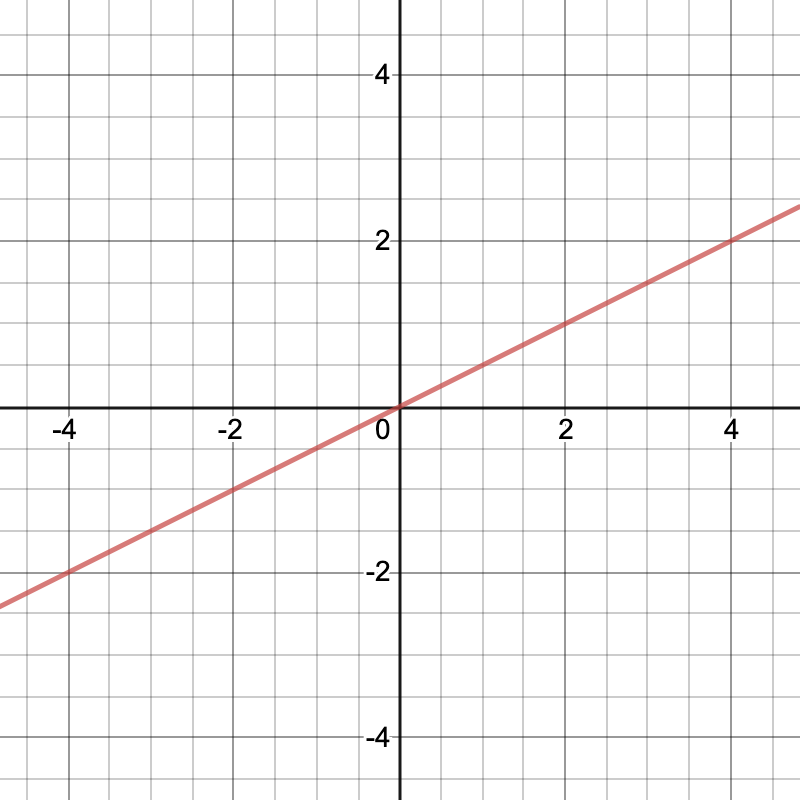
\includegraphics[scale=0.1]{a}
    б)$y=\sqrt{x+1}$
    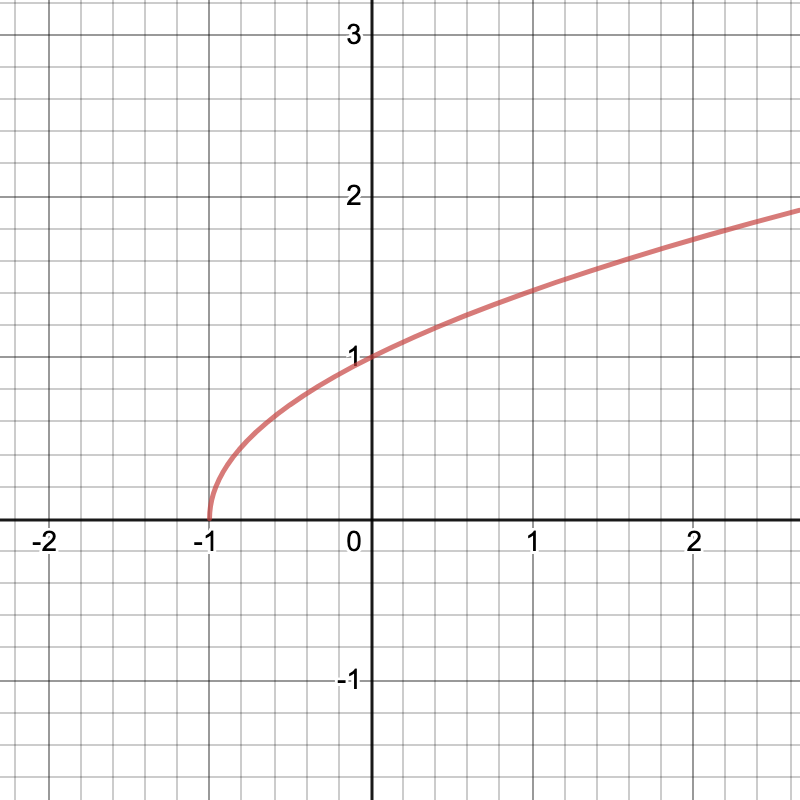
\includegraphics[scale=0.1]{b}\\
    в)$y=ln(x-1)$
    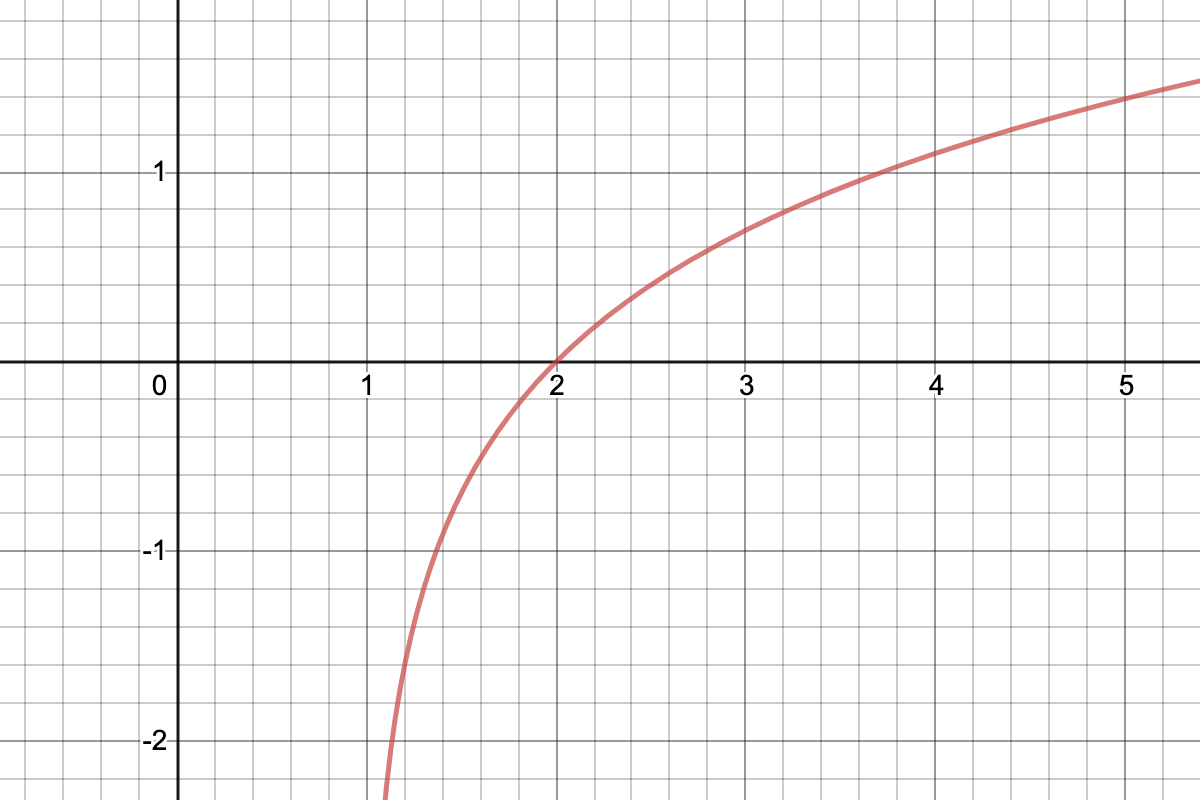
\includegraphics[scale=0.1]{c}
    г)$y=-sinx$
    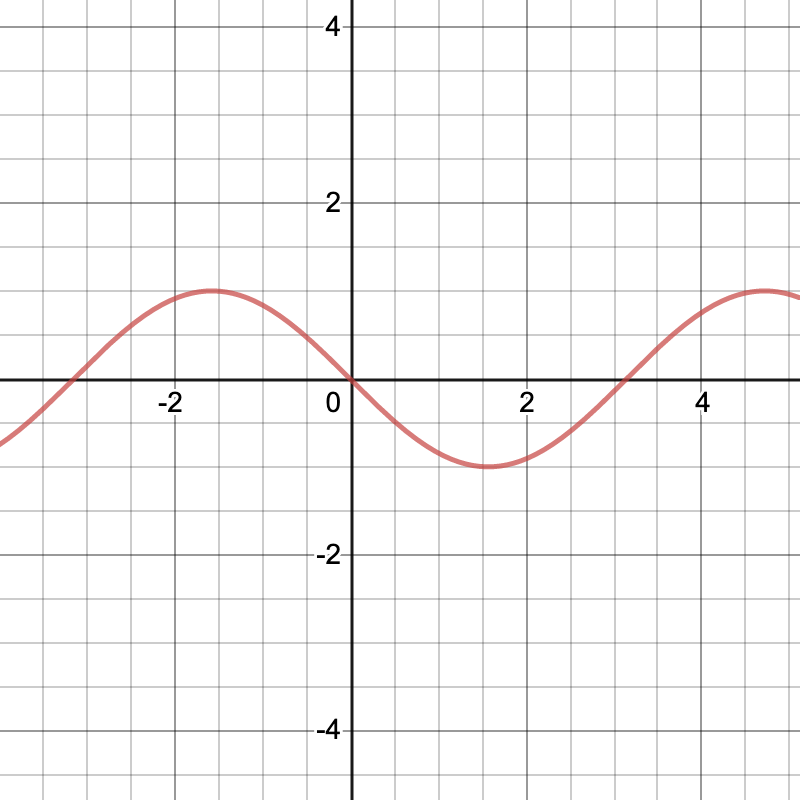
\includegraphics[scale=0.1]{d}\\
    д)$y=cos2x$
    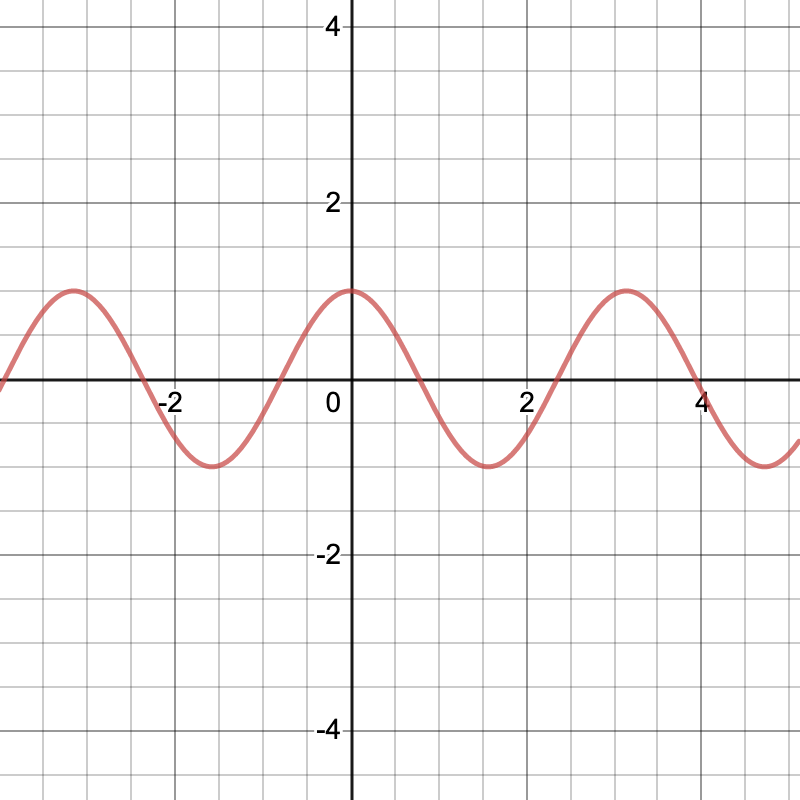
\includegraphics[scale=0.1]{e}
    е)$y=ctg2x$
    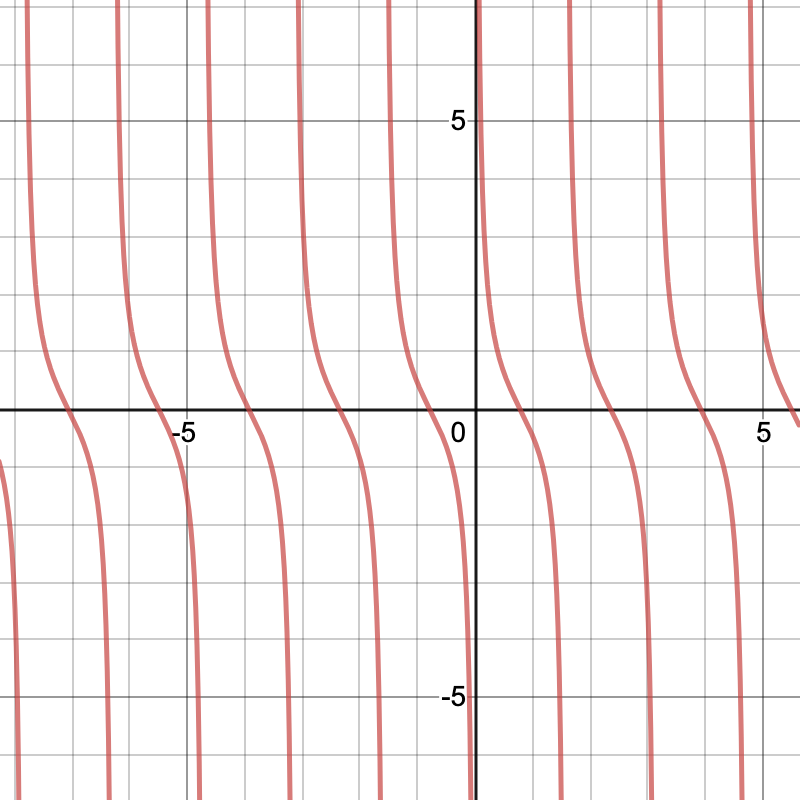
\includegraphics[scale=0.1]{f}\\
    ё)$y=arcsin\frac{x}{2}$
    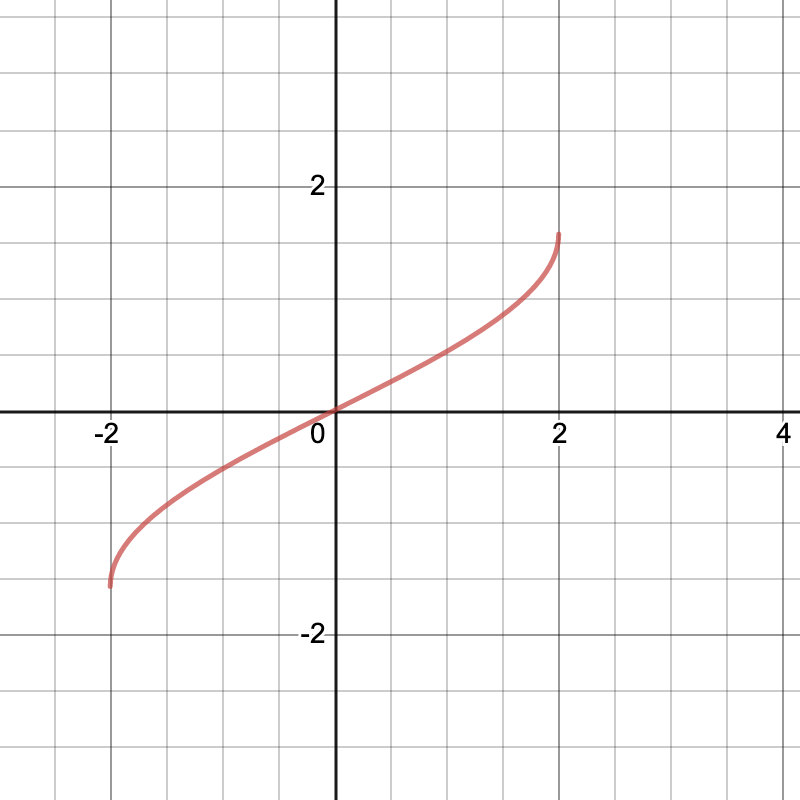
\includegraphics[scale=0.1]{g}
    ж)$y=arctg2x$
    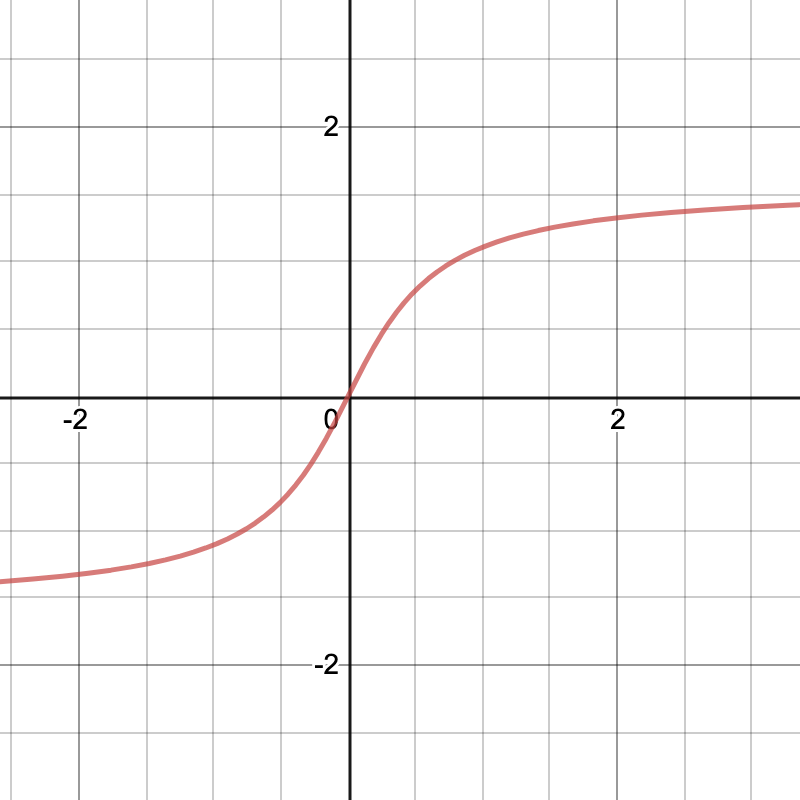
\includegraphics[scale=0.1]{h}\\
    и)$y=arcctg(-x)$
    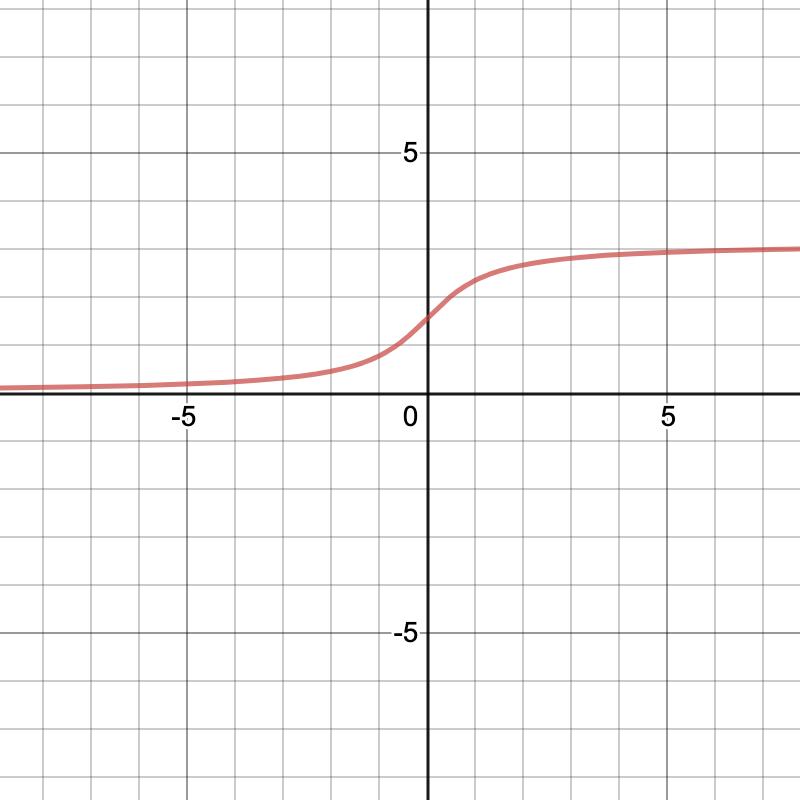
\includegraphics[scale=0.1]{i}\\\\
    2)$\lim\frac{n(2-n)}{5+3n+2n^2}
    =\lim\frac{2n-n^2}{5+3n+2n^2}
    =\lim\frac{2-2n}{3+4n}
    =\lim\frac{2}{4}
    -\frac{1}{2}$\\
    3)$\lim\frac{\sqrt{n^3}-1}{n(n-3)}
    =\lim\frac{n^\frac{3}{2}-1}{n^2-3n}
    =\lim\frac{\frac{3}{2}n^\frac{1}{2}}{2n-3}
    =\lim\frac{\frac{3}{4}b^{-\frac{1}{2}}}{2}
    =\lim\frac{3}{8b^\frac{1}{2}}=0$\\
    4)$\lim\frac{n^2}{\sqrt{n^3+1}}
    =\lim\frac{2}{\frac{1}{2}(n^3+1)^{-\frac{1}{2}}(3n)}
    =\lim\frac{4\sqrt{n^3+1}}{3n}=+\infty$\\
    5)$\lim\limits_{x\to -2}\frac{4-x^2}{x^2+x-2}
    =\lim\limits_{x\to -2}\frac{-2x}{2x+1}
    =-\frac{4}{3}$\\
    6)$\lim\limits_{x\to \frac{\pi}{2}}\frac{x}{cosx}
    =\frac{\frac{\pi}{2}}{0}=\infty$\\
    7)$\lim\limits_{x\to 1}\frac{x^2-1}{(x-1)^2}
    =\lim\limits_{x\to 1}\frac{(x+1)}{(x-1)}=\infty$\\
    8)$\lim\limits_{x\to 0}\frac{sin3x}{x-2x^2}
    =\lim\limits_{x\to 0}\frac{3x}{x-2x^2}
    \lim\limits_{x\to 0}\frac{3}{1-4x}
    =\lim\limits_{x\to 0}\frac{3}{1}
    =3$\\
    9)$\lim\limits_{x\to 0}xctg2x
    =\lim\limits_{x\to 0}\frac{x}{tg2x}
    =\lim\limits_{x\to 0}\frac{1}{2}
    =\frac{1}{2}$\\
    10)$\lim\limits_{x\to \infty}\frac{x-3x^2}{2x^2-1}
    =\lim\limits_{x\to \infty}\frac{\frac{1}{x}-3}{2-\frac{1}{x^2}}
    =-\frac{3}{2}$\\
    11)$11$\\
    12)Найдите приращение функции $y=\sqrt{1+x^2}$ в точке $x=0$, если $\Delta x=-\frac{3}{4}$.\\
    $\Delta y=f(x_0+\Delta x)-f(x_0)$\\
    $\Delta y=\sqrt{1+(0-\frac{3}{4})^2}-\sqrt{1+0^2}$\\
    $\Delta y=\frac{5}{4}-1=\frac{1}{4}$\\
    13)\\
    14)\\
    15)$f(x)=x^4+x. \lim\limits_{\Delta x\to 0}\frac{f(-1+\Delta x)-f(-1)}{\Delta x}$\\
    $f'(x)=4x^3+1$\\
    $f'(-1)=4(-1^3)+1=-3$\\
    16)\\
    17)\\
    18)$y=x^2\sqrt{1-x^2}.$\\
    $y'=2x\sqrt{1-x^2}+\frac{2x^3}{2\sqrt{1-x^2}}
    =\frac{4x^2(1-x^2)+2x^3}{2x\sqrt{1-x^2}}
    =\frac{}{}$



\end{document}